% Options for packages loaded elsewhere
\PassOptionsToPackage{unicode}{hyperref}
\PassOptionsToPackage{hyphens}{url}
%
\documentclass[
]{article}
\usepackage{amsmath,amssymb}
\usepackage{iftex}
\ifPDFTeX
  \usepackage[T1]{fontenc}
  \usepackage[utf8]{inputenc}
  \usepackage{textcomp} % provide euro and other symbols
\else % if luatex or xetex
  \usepackage{unicode-math} % this also loads fontspec
  \defaultfontfeatures{Scale=MatchLowercase}
  \defaultfontfeatures[\rmfamily]{Ligatures=TeX,Scale=1}
\fi
\usepackage{lmodern}
\ifPDFTeX\else
  % xetex/luatex font selection
\fi
% Use upquote if available, for straight quotes in verbatim environments
\IfFileExists{upquote.sty}{\usepackage{upquote}}{}
\IfFileExists{microtype.sty}{% use microtype if available
  \usepackage[]{microtype}
  \UseMicrotypeSet[protrusion]{basicmath} % disable protrusion for tt fonts
}{}
\makeatletter
\@ifundefined{KOMAClassName}{% if non-KOMA class
  \IfFileExists{parskip.sty}{%
    \usepackage{parskip}
  }{% else
    \setlength{\parindent}{0pt}
    \setlength{\parskip}{6pt plus 2pt minus 1pt}}
}{% if KOMA class
  \KOMAoptions{parskip=half}}
\makeatother
\usepackage{xcolor}
\usepackage[margin=1in]{geometry}
\usepackage{color}
\usepackage{fancyvrb}
\newcommand{\VerbBar}{|}
\newcommand{\VERB}{\Verb[commandchars=\\\{\}]}
\DefineVerbatimEnvironment{Highlighting}{Verbatim}{commandchars=\\\{\}}
% Add ',fontsize=\small' for more characters per line
\usepackage{framed}
\definecolor{shadecolor}{RGB}{248,248,248}
\newenvironment{Shaded}{\begin{snugshade}}{\end{snugshade}}
\newcommand{\AlertTok}[1]{\textcolor[rgb]{0.94,0.16,0.16}{#1}}
\newcommand{\AnnotationTok}[1]{\textcolor[rgb]{0.56,0.35,0.01}{\textbf{\textit{#1}}}}
\newcommand{\AttributeTok}[1]{\textcolor[rgb]{0.13,0.29,0.53}{#1}}
\newcommand{\BaseNTok}[1]{\textcolor[rgb]{0.00,0.00,0.81}{#1}}
\newcommand{\BuiltInTok}[1]{#1}
\newcommand{\CharTok}[1]{\textcolor[rgb]{0.31,0.60,0.02}{#1}}
\newcommand{\CommentTok}[1]{\textcolor[rgb]{0.56,0.35,0.01}{\textit{#1}}}
\newcommand{\CommentVarTok}[1]{\textcolor[rgb]{0.56,0.35,0.01}{\textbf{\textit{#1}}}}
\newcommand{\ConstantTok}[1]{\textcolor[rgb]{0.56,0.35,0.01}{#1}}
\newcommand{\ControlFlowTok}[1]{\textcolor[rgb]{0.13,0.29,0.53}{\textbf{#1}}}
\newcommand{\DataTypeTok}[1]{\textcolor[rgb]{0.13,0.29,0.53}{#1}}
\newcommand{\DecValTok}[1]{\textcolor[rgb]{0.00,0.00,0.81}{#1}}
\newcommand{\DocumentationTok}[1]{\textcolor[rgb]{0.56,0.35,0.01}{\textbf{\textit{#1}}}}
\newcommand{\ErrorTok}[1]{\textcolor[rgb]{0.64,0.00,0.00}{\textbf{#1}}}
\newcommand{\ExtensionTok}[1]{#1}
\newcommand{\FloatTok}[1]{\textcolor[rgb]{0.00,0.00,0.81}{#1}}
\newcommand{\FunctionTok}[1]{\textcolor[rgb]{0.13,0.29,0.53}{\textbf{#1}}}
\newcommand{\ImportTok}[1]{#1}
\newcommand{\InformationTok}[1]{\textcolor[rgb]{0.56,0.35,0.01}{\textbf{\textit{#1}}}}
\newcommand{\KeywordTok}[1]{\textcolor[rgb]{0.13,0.29,0.53}{\textbf{#1}}}
\newcommand{\NormalTok}[1]{#1}
\newcommand{\OperatorTok}[1]{\textcolor[rgb]{0.81,0.36,0.00}{\textbf{#1}}}
\newcommand{\OtherTok}[1]{\textcolor[rgb]{0.56,0.35,0.01}{#1}}
\newcommand{\PreprocessorTok}[1]{\textcolor[rgb]{0.56,0.35,0.01}{\textit{#1}}}
\newcommand{\RegionMarkerTok}[1]{#1}
\newcommand{\SpecialCharTok}[1]{\textcolor[rgb]{0.81,0.36,0.00}{\textbf{#1}}}
\newcommand{\SpecialStringTok}[1]{\textcolor[rgb]{0.31,0.60,0.02}{#1}}
\newcommand{\StringTok}[1]{\textcolor[rgb]{0.31,0.60,0.02}{#1}}
\newcommand{\VariableTok}[1]{\textcolor[rgb]{0.00,0.00,0.00}{#1}}
\newcommand{\VerbatimStringTok}[1]{\textcolor[rgb]{0.31,0.60,0.02}{#1}}
\newcommand{\WarningTok}[1]{\textcolor[rgb]{0.56,0.35,0.01}{\textbf{\textit{#1}}}}
\usepackage{graphicx}
\makeatletter
\def\maxwidth{\ifdim\Gin@nat@width>\linewidth\linewidth\else\Gin@nat@width\fi}
\def\maxheight{\ifdim\Gin@nat@height>\textheight\textheight\else\Gin@nat@height\fi}
\makeatother
% Scale images if necessary, so that they will not overflow the page
% margins by default, and it is still possible to overwrite the defaults
% using explicit options in \includegraphics[width, height, ...]{}
\setkeys{Gin}{width=\maxwidth,height=\maxheight,keepaspectratio}
% Set default figure placement to htbp
\makeatletter
\def\fps@figure{htbp}
\makeatother
\setlength{\emergencystretch}{3em} % prevent overfull lines
\providecommand{\tightlist}{%
  \setlength{\itemsep}{0pt}\setlength{\parskip}{0pt}}
\setcounter{secnumdepth}{-\maxdimen} % remove section numbering
\ifLuaTeX
  \usepackage{selnolig}  % disable illegal ligatures
\fi
\usepackage{bookmark}
\IfFileExists{xurl.sty}{\usepackage{xurl}}{} % add URL line breaks if available
\urlstyle{same}
\hypersetup{
  pdftitle={DATA 621 - Group Assignment 3 Write Up: Logistic Regression on Crime Rates: Write Up},
  pdfauthor={(Group 4) Eddie Xu, Mohamed Hassan-El Serafi, Chun Shing Leung, Keith Colella, Yina, Qiao},
  hidelinks,
  pdfcreator={LaTeX via pandoc}}

\title{DATA 621 - Group Assignment 3 Write Up: Logistic Regression on
Crime Rates: Write Up}
\author{(Group 4) Eddie Xu, Mohamed Hassan-El Serafi, Chun Shing Leung,
Keith Colella, Yina, Qiao}
\date{2024-11-03}

\begin{document}
\maketitle

{
\setcounter{tocdepth}{3}
\tableofcontents
}
\section{Introduction}\label{introduction}

Crime rates in neighborhoods are an important factor in finding a new
home or allocating resources to better improve the affected
neighborhood. For this assignment, our group are going to explore,
analyze and model a data set containing information on crime for various
neighborhoods of a major city and later going to use binary logistic
regression to predict whether the neighborhood will be at risk for high
crime levels. A binary logistic regression is a statistic method that
models the relation between a binary dependent variable and a set of
independent variables. It is widely used to determine dichotomous
outcomes.

In this assignment, our group explored the training data set for better
understanding. We later prepared the data based on the insight and
produced 3 different training data sets. After that, we evaluated all
binary models and determined the best model that offers the best
accuracy and completeness.

\section{Data Exploration}\label{data-exploration}

\emph{Describe the size and the variables in the crime training data
set. Consider that too much detail will cause a manager to lose interest
while too little detail will make the manager consider that you aren't
doing your job.}

A simple exploratory data analysis will be conducted and the training
data provided will be used to determine the property and value of the
dataset. The \texttt{DataExplorer} package will be used to provide a
full profile for the data frame.

\subsubsection{Data Set}\label{data-set}

With the data set given, there are 466 rows, 13 columns and 6058
observations. There is no missing values or observations and all columns
have continuous values. The \texttt{chas} variable is the only dummy
variable out of 13 columns and is used to determine if the suburb
borders the Charles River. Based on the histograms, both \texttt{rm} and
\texttt{medv} variables are normally distributed, while other variables
are skewed. Both tax and rad variables have a large proportion of
outliers. Specifically, 121 of the 466 total observations have the same
values that appear outside the normal range of each variable. The value
\texttt{666} is used for \texttt{tax} and \texttt{24} for \texttt{rad}.
We suspect these values may be constant placeholders, indicating a
potential data quality issue. We decided not to create new variables
because there is not enough relevant information in the data set to
suggest new variables might be needed.

\begin{figure}
\centering
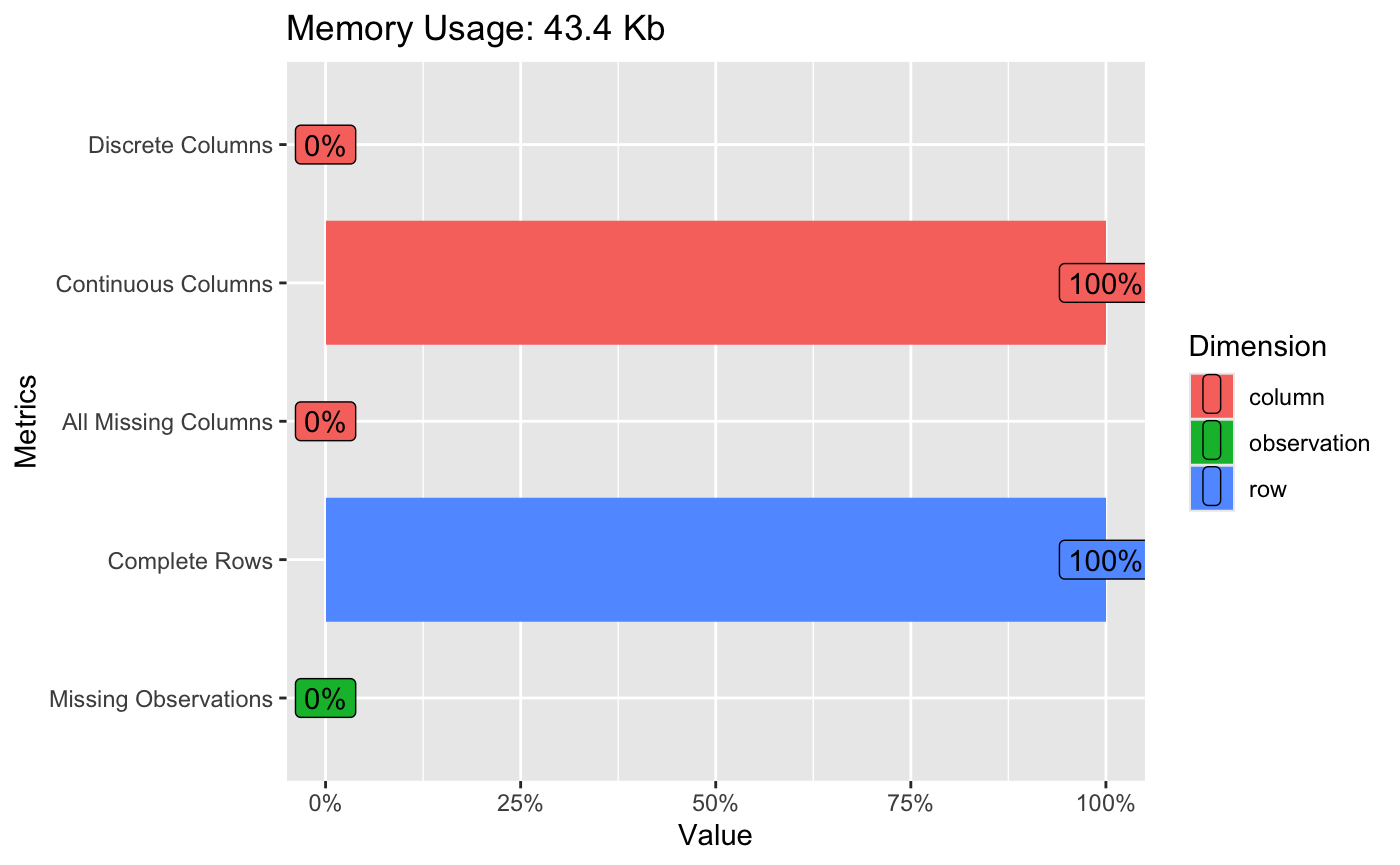
\includegraphics{/Users/mohamedhassan/Downloads/hw3_metrics_plot.png}
\caption{Metrics}
\end{figure}

\begin{figure}
\centering
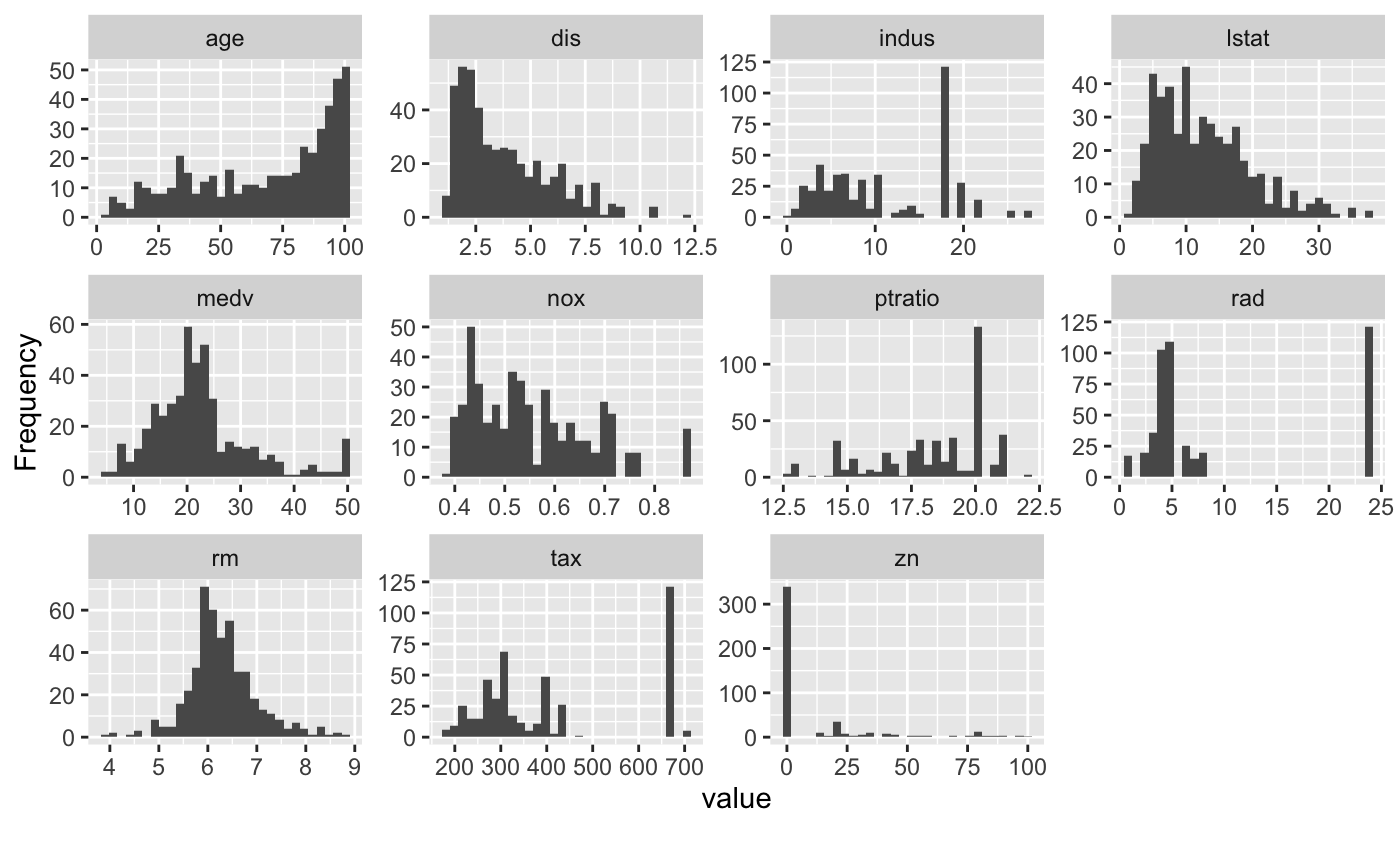
\includegraphics{/Users/mohamedhassan/Downloads/hw3_hist_plot.png}
\caption{Histogram}
\end{figure}

The box plots highlight the median of each variable when divided into
subsets according to the target variable's two classes. The plot
demonstrate that, for most variables, there is a clear difference in the
median values across each class. This would indicate that these
variables are likely to provide meaningful signal in predicting the
target label.

\begin{figure}
\centering
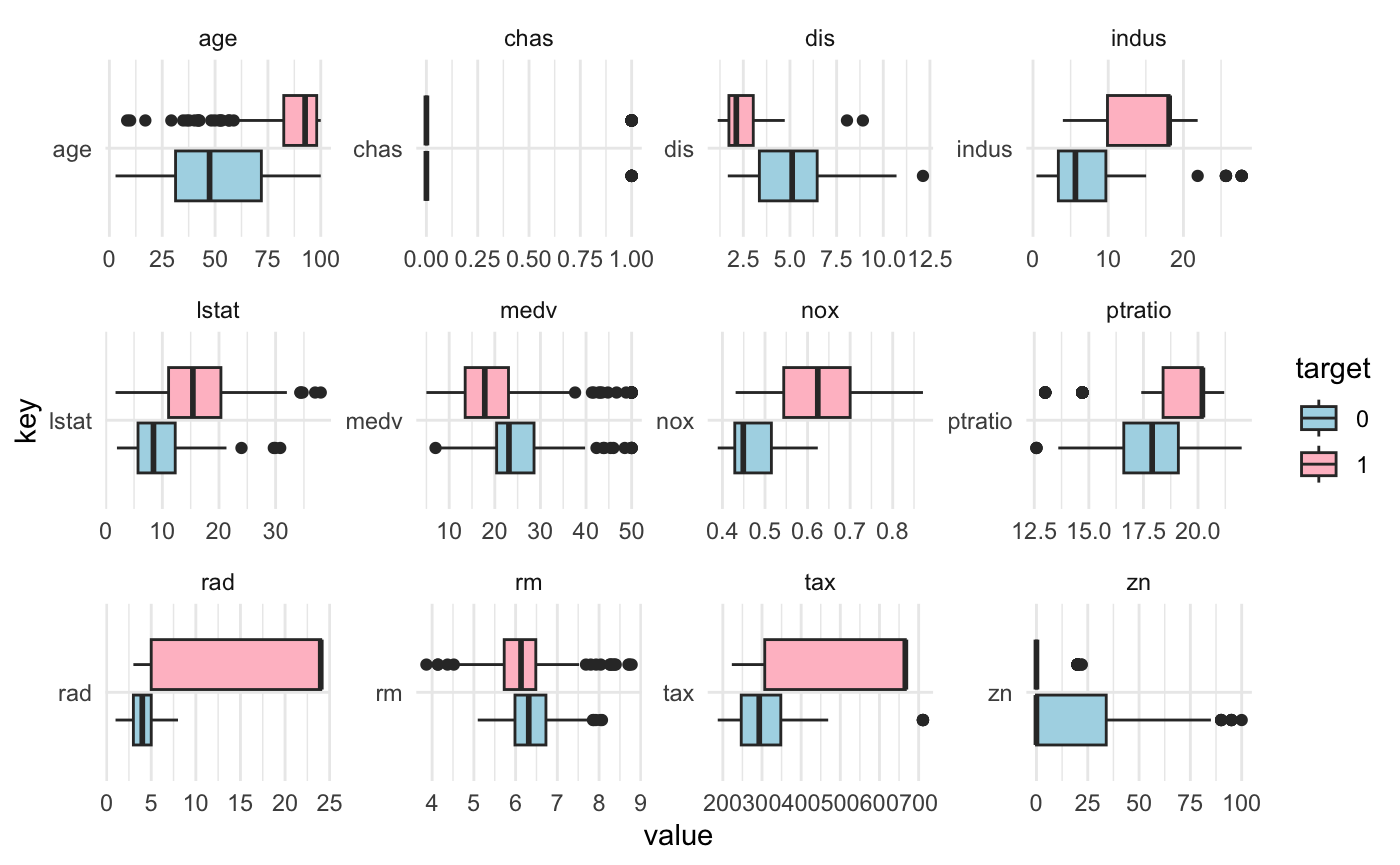
\includegraphics{/Users/mohamedhassan/Downloads/hw3_boxplot.png}
\caption{Boxplot}
\end{figure}

Based on the correlation plot, it shows that \texttt{rad} and
\texttt{dis} have the highest positive correlation compared to other
variables.

\begin{figure}
\centering
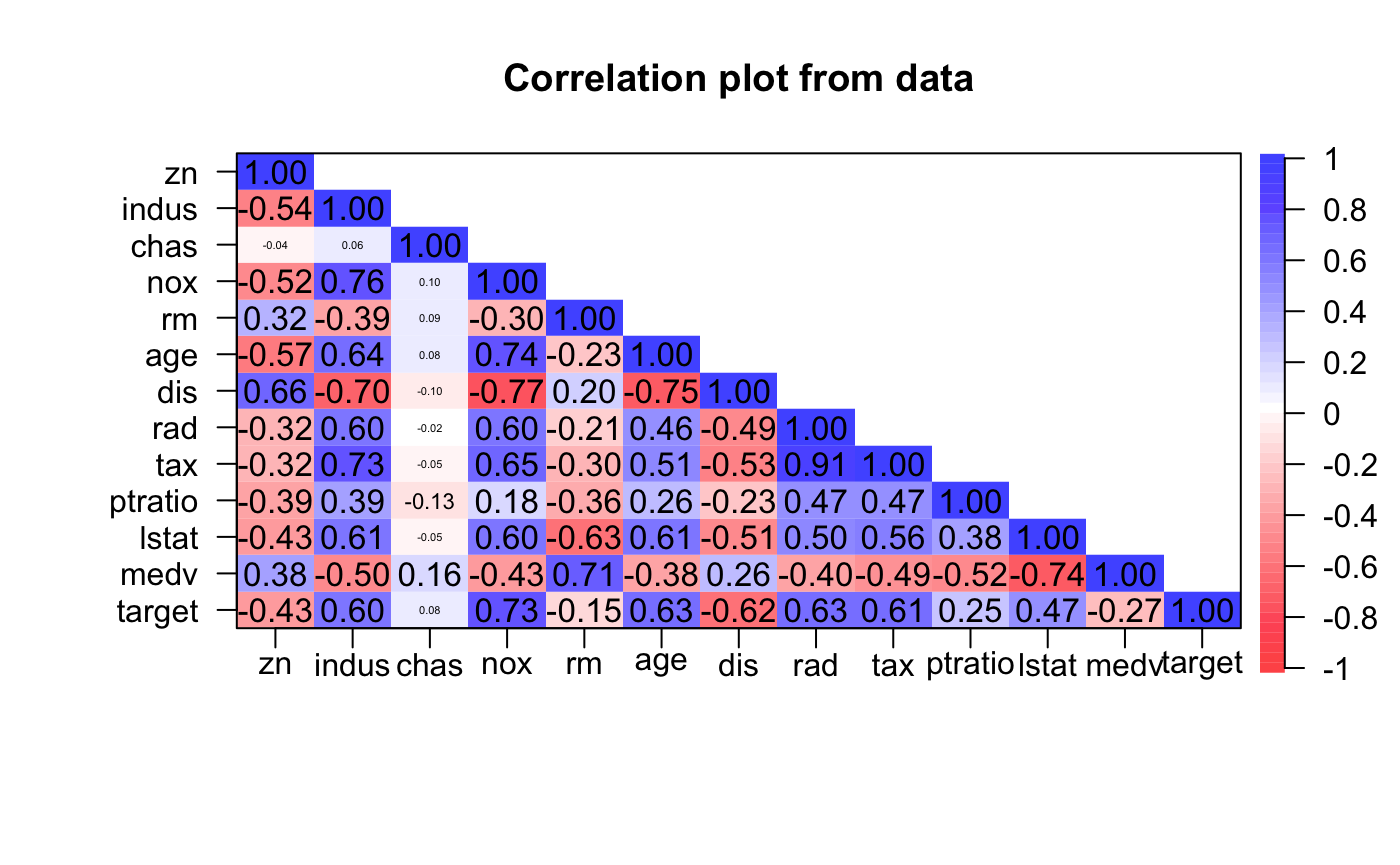
\includegraphics{/Users/mohamedhassan/Downloads/hw3_corr_plot.png}
\caption{Correlation Plot}
\end{figure}

To determine if the dataset is compatible with the binary logistic
regression model, the model is fitted and the VIF score analysis is
conducted to check for any multicollinearity.

After the model fitting, the P-value of the F-statistic is less than
0.05, showing that predictor variables may be significantly associated
with the outcome. There are variables in the data set with moderate
correlation between predictor variables. Both \texttt{rad} and
\texttt{tax} variables have the highest VIF scores and it is over 5,
showing that they are severely correlated with other predictor
variables. Therefore, either variable need to removed and need to
reevaluated before modeling the binary regression model.

With either \texttt{rad} or \texttt{tax} variables removed from the data
set, the updated data set is reevaluated and with the updated VIF score,
both variable score dropped below 5 and it appears that \texttt{tax}
variable have a bigger impact. Therefore, the data set with \texttt{tax}
removed will be selected for the model building.

\section{Data Preparation}\label{data-preparation}

\emph{Describe how you have transformed the data by changing the
original variables or creating new variables. If you did transform the
data or create new variables, discuss why you did this.}

Based on the outcome from our data exploratory analysis, some of the
variables are identified to be skewed, so log transformations are needed
to address the issue. Log transformations are applied on these
variables: \texttt{lstat}, \texttt{age}, \texttt{indus}, \texttt{tax},
\texttt{rad} and \texttt{dis}. This method can reduce the skewness of
the data and diminish the impact of outliers in variables such as
\texttt{indus}, \texttt{tax}, and \texttt{rad} since they have a large
population of outliers. With the log transformed variables, the original
variables are removed from the data set.

Since \texttt{tax} and \texttt{rad} variables have outliers, those
outliers will be removed given that they might be a data quality issue.
Since there is no additional information about these outliers, they are
considered to be removed so the model will not be affected by those
outliers.

\section{Build Model}\label{build-model}

\emph{Using the training data, build at least three different binary
logistic regression models, using different variables (or the same
variables with different transformations). You may select the variables
manually, use an approach such as Forward or Step wise, use a different
approach, or use a combination of techniques. Describe the techniques
you used. If you manually selected a variable for inclusion into the
model or exclusion into the model, indicate why this was done. Be sure
to explain how you can make inferences from the model, as well as
discuss other relevant model output.}

With the training data explored and prepped, 4 different models were
built to determine the best model. The first model is based on the
original training data set and will set the baseline. From there, we can
compare other 3 models and see any improvement.

The second data set is based on the log transformation on skewed
variables and the original skewed variables removed. With that, we can
expect the model to be significantly improved than the first model.

The third data set is derived from the original dataset and the
\texttt{tax} variable being removed and there was no log transformation
on the skewed variables. Since the \texttt{tax} variables have a bigger
impact, it will be removed and we can expect the model will be improved
than the first model.

The last model will be based on a dataset with rows removed due to them
being outliers on \texttt{tax} and \texttt{rad} variables. Since the
value \texttt{666} is used for \texttt{tax} and \texttt{24} for
\texttt{rad} and with no additional relevant information, we decided to
remove them to see if the variables without those outliers will perform
better than the second model with the log transformation on those
variables.

\section{Select Model}\label{select-model}

\emph{Decide on the criteria for selecting the best binary logistic
regression model. Will you select models with slightly worse performance
if it makes more sense or is more parsimonious? Discuss why you selected
your model.}

In order to select the best model, we decided to use the confusion
matrix(accuracy), the F-1 score, and ROC curve to help analyze each
model's performance. The confusion matrix provides a better
understanding in the model's prediction, especially the accuracy part.
The accuracy from the confusion matrix represents how accurate is the
model's prediction and it is a common method to evaluate the model. The
F-1 score is the balanced measure of both precision and recall and it
will help us to assess the model's performance. The ROC curve visualizes
how well the model distinguish each variables and the AUC outcome can
demonstrates how well the model can classify the positive and negative
results.

For the first model, AUC score is 98.86\%, the accuracy is 0.9355 and
the F-1 Score is 0.9423. By comparing the first model to other models,
we saw different changes in those models.

\begin{figure}
\centering
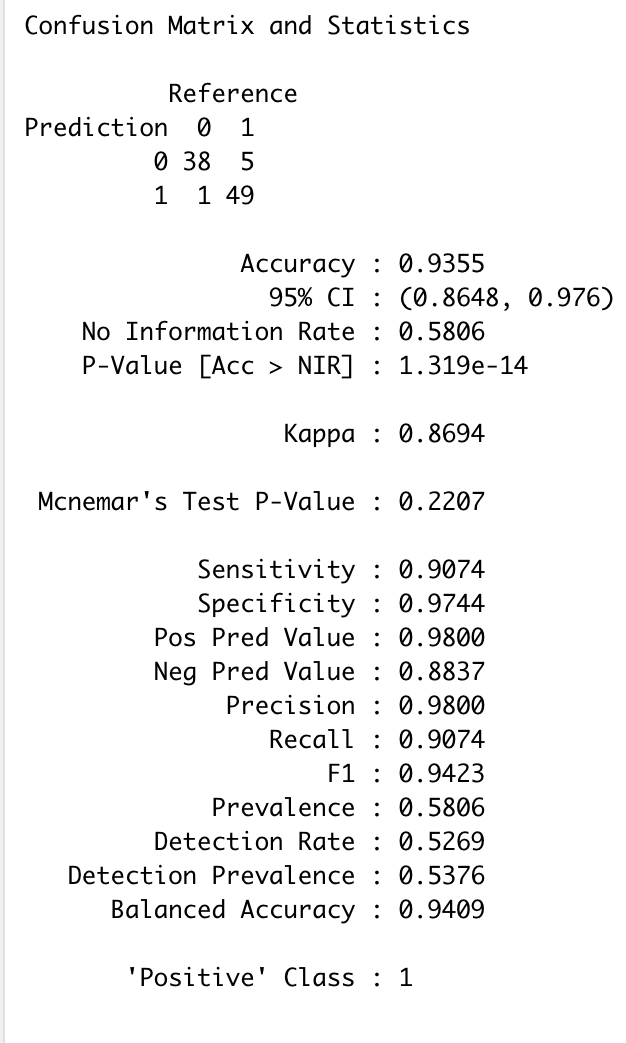
\includegraphics{/Users/mohamedhassan/Documents/HW3 CM SS Model 1.png}
\caption{Model 1 Confusion Matrix Statistics}
\end{figure}

\begin{figure}
\centering
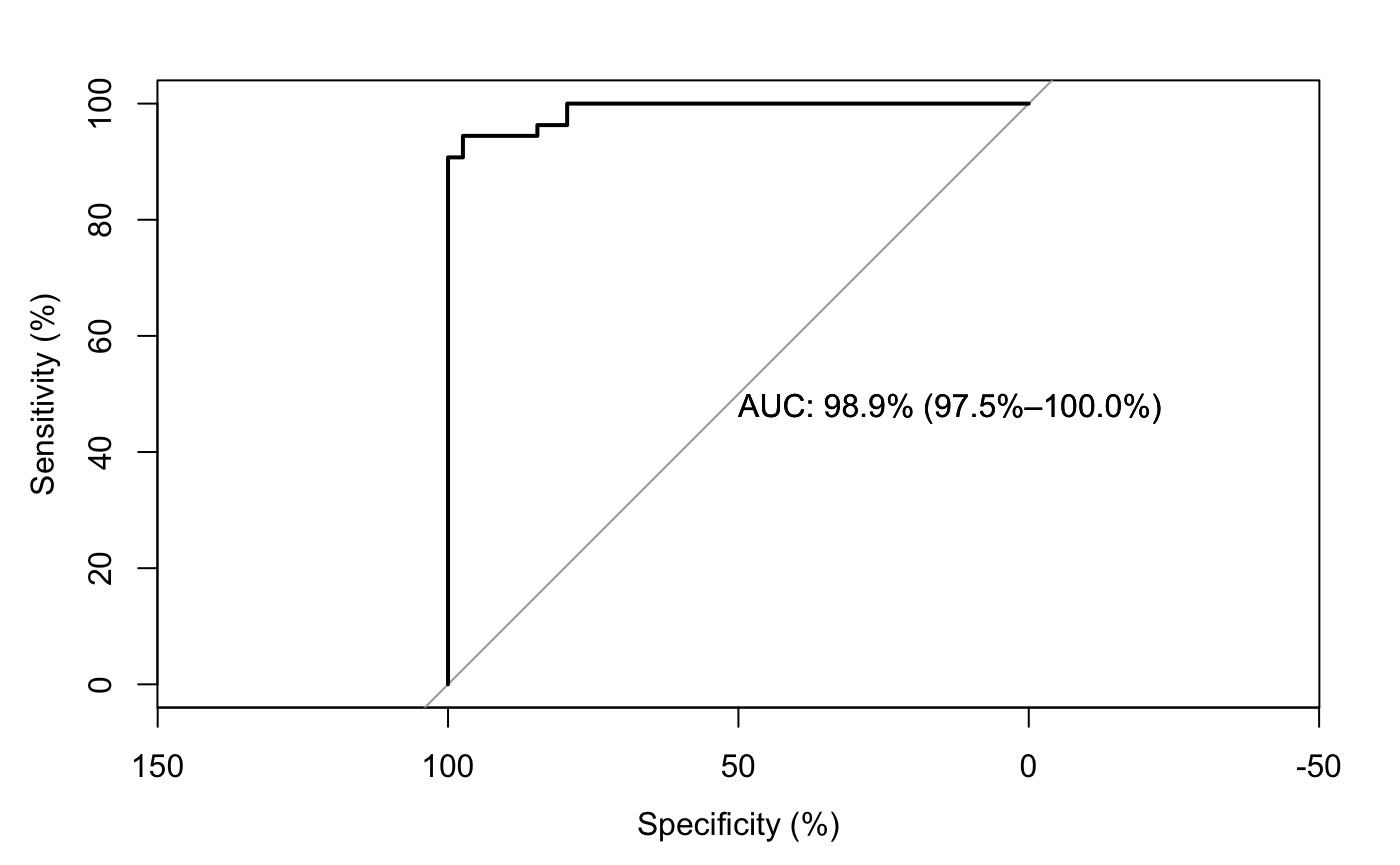
\includegraphics{/Users/mohamedhassan/Downloads/hw3_roc_curve1.png}
\caption{Model 1 ROC Curve}
\end{figure}

The second model with the log transformation have the AUC score of
98.53\%, the F-1 Score of 0.9216 and the accuracy of 0.914. Compared to
the first model, this is an unexpected result. All metric from the
second model slightly deteriorated.

\begin{figure}
\centering
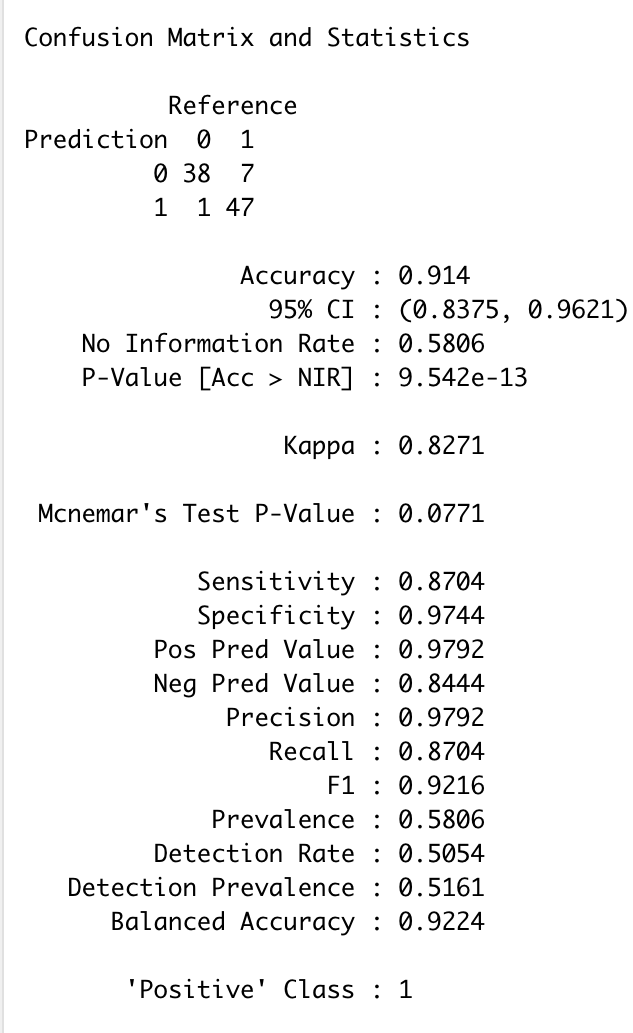
\includegraphics{/Users/mohamedhassan/Documents/HW3 CM SS Model 2.png}
\caption{Model 2 Confusion Matrix Statistics}
\end{figure}

\begin{figure}
\centering
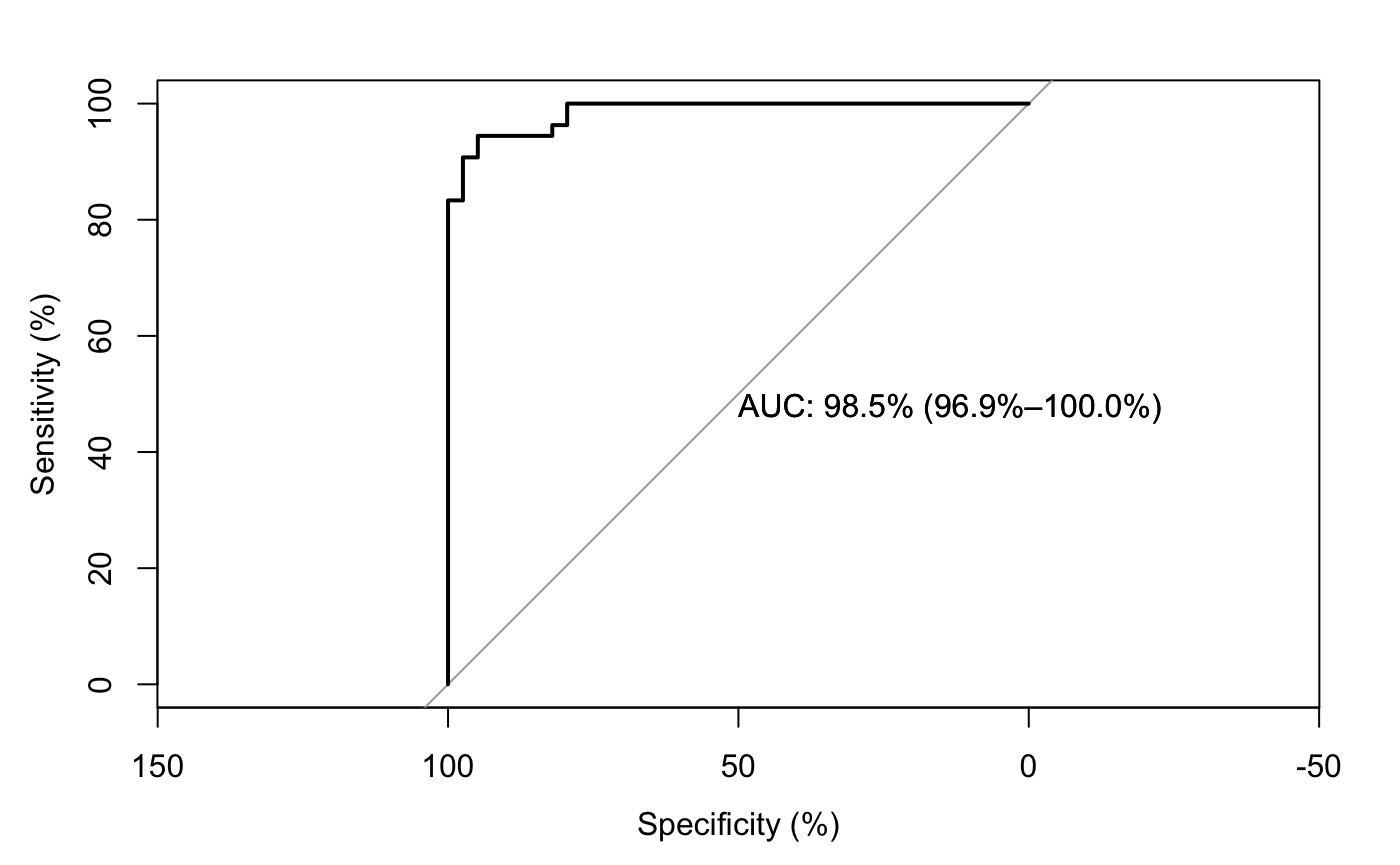
\includegraphics{/Users/mohamedhassan/Downloads/hw3_roc_curve2.png}
\caption{Model 2 ROC Curve}
\end{figure}

The third model with \texttt{tax} variable removed slightly deteriorated
compared to the first model. The AUC for that model is 98.67, the
accuracy is 0.9355 and the F-1 Score is 0.9268.

\begin{figure}
\centering
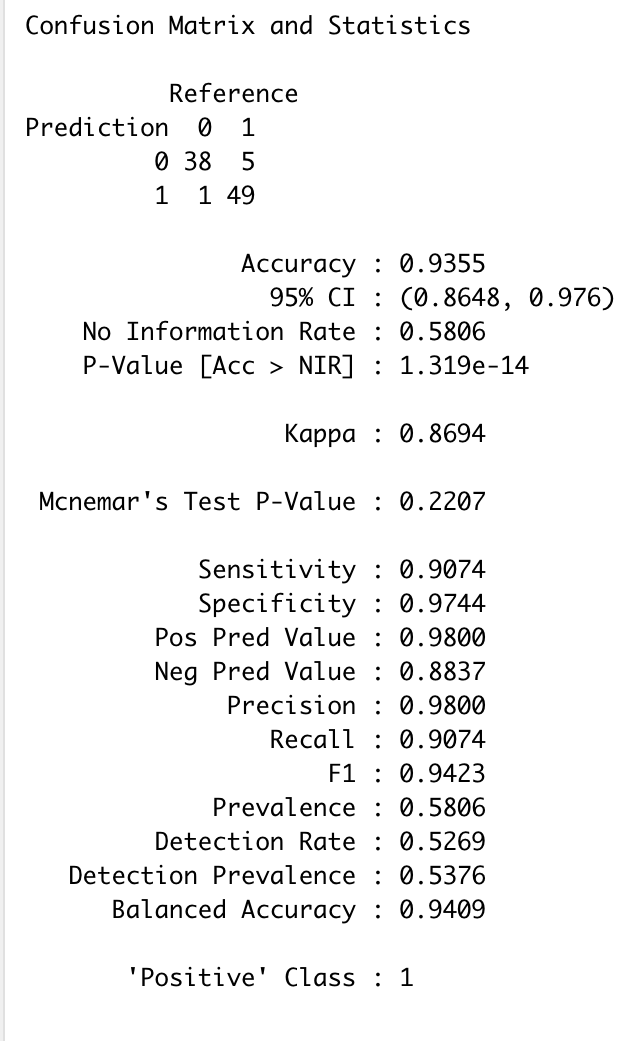
\includegraphics{/Users/mohamedhassan/Documents/HW3 CM SS Model 3.png}
\caption{Model 3 Confusion Matrix Statistics}
\end{figure}

\begin{figure}
\centering
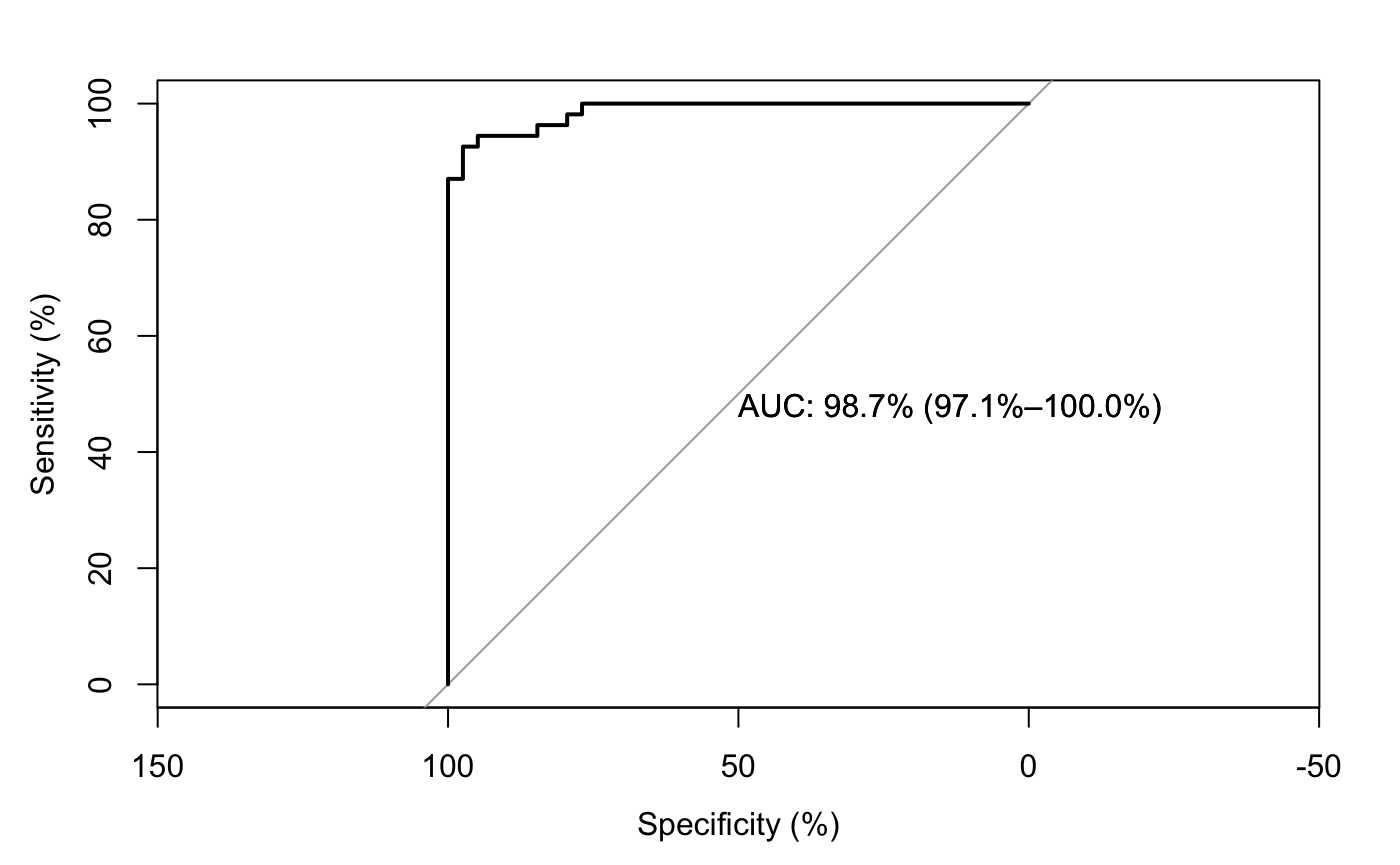
\includegraphics{/Users/mohamedhassan/Downloads/hw3_roc_curve3.png}
\caption{Model 3 ROC Curve}
\end{figure}

The last model with all outliers removed have the worst result from all
metrics. The F-1 Score is 0.6000, the accuracy is 0.8261 an the AUC is
92.72\%, making the model with the worst performance.

\begin{figure}
\centering
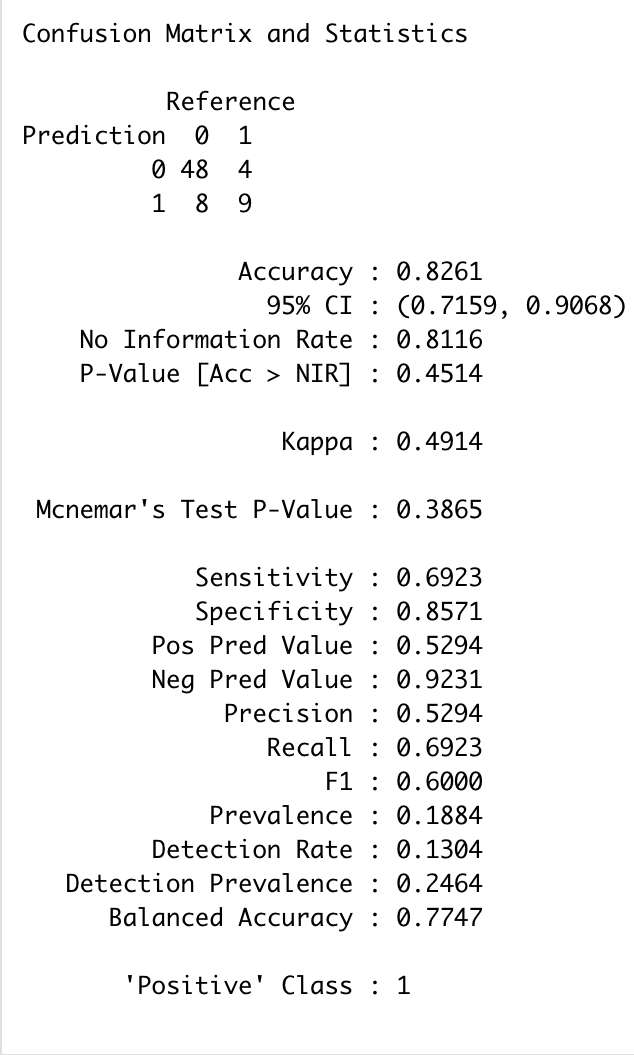
\includegraphics{/Users/mohamedhassan/Documents/HW3 CM SS Model 4.png}
\caption{Model 4 Confusion Matrix Statistics}
\end{figure}

\begin{figure}
\centering
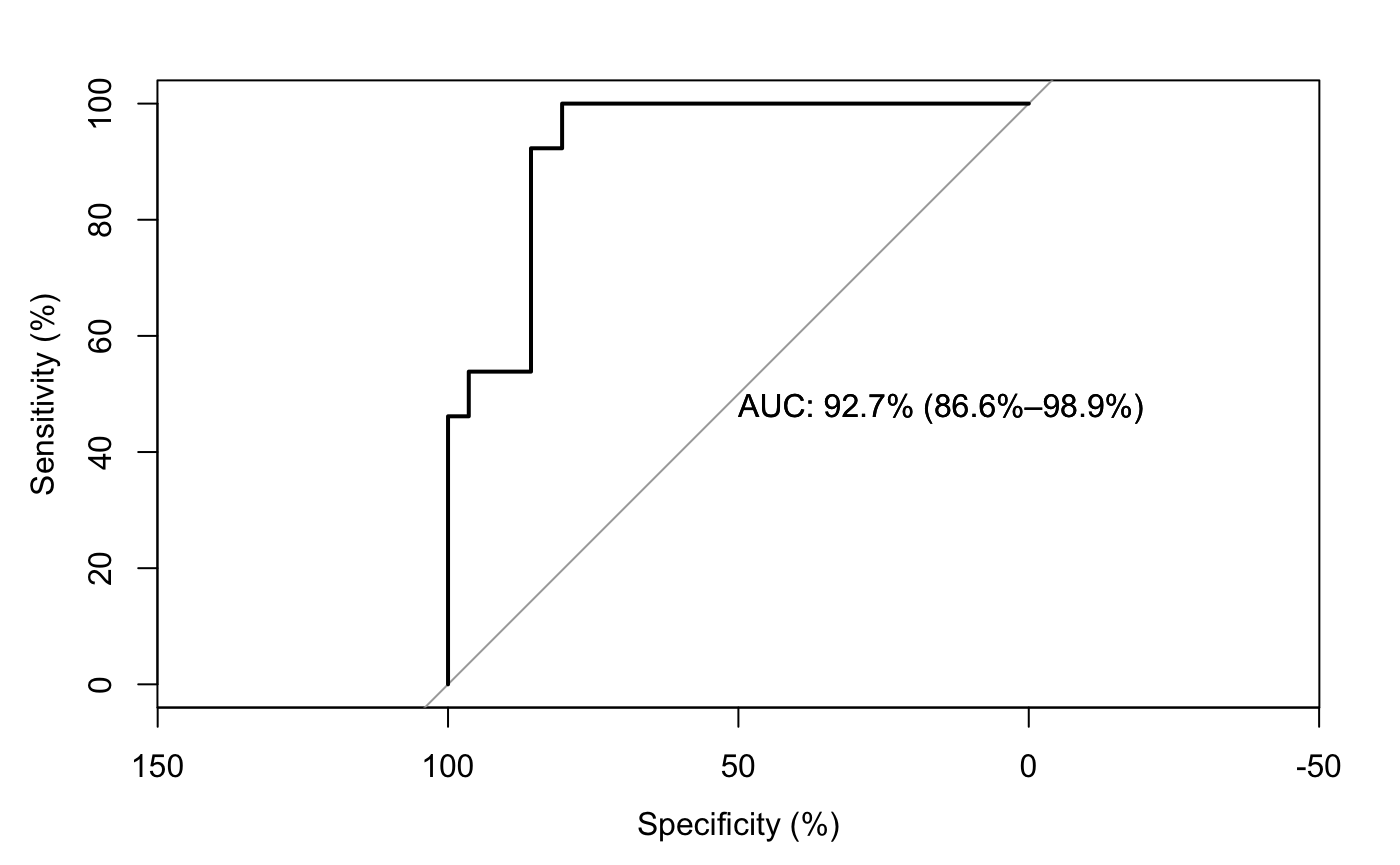
\includegraphics{/Users/mohamedhassan/Downloads/hw3_roc_curve4.png}
\caption{Model 4 ROC Curve}
\end{figure}

Out of all models, we decided to select the second model with the log
transformation. Both first and third models have better performance and
metric results than the second model, but the data used in those models
have outliers, which can impact the model's prediction and making it
harder to generalize the result. This could lead to unreliable
predictions.

\section{Appendix}\label{appendix}

\begin{Shaded}
\begin{Highlighting}[]
\DocumentationTok{\#\#  Data Exploration}
\CommentTok{\# pull in the training data set}
\NormalTok{crime\_training\_data }\OtherTok{\textless{}{-}} \FunctionTok{read.csv}\NormalTok{(}\StringTok{"https://raw.githubusercontent.com/eddiexunyc/crime\_binary\_logistic\_regression/refs/heads/main/Resources/crime{-}training{-}data\_modified.csv"}\NormalTok{)}

\CommentTok{\# pull in the test data}
\NormalTok{crime\_test\_data }\OtherTok{\textless{}{-}} \FunctionTok{read.csv}\NormalTok{(}\StringTok{"https://raw.githubusercontent.com/eddiexunyc/crime\_binary\_logistic\_regression/refs/heads/main/Resources/crime{-}evaluation{-}data\_modified.csv"}\NormalTok{)}

\FunctionTok{glimpse}\NormalTok{(crime\_training\_data)}

\FunctionTok{introduce}\NormalTok{(crime\_training\_data)}

\CommentTok{\# par on plots}
\FunctionTok{par}\NormalTok{(}\AttributeTok{mfrow =} \FunctionTok{c}\NormalTok{(}\DecValTok{1}\NormalTok{, }\DecValTok{4}\NormalTok{))}
\FunctionTok{plot\_intro}\NormalTok{(crime\_training\_data)}
\FunctionTok{describeBy}\NormalTok{(crime\_training\_data)}
\FunctionTok{plot\_histogram}\NormalTok{(crime\_training\_data)}

\CommentTok{\# boxplot on variables}
\NormalTok{crime\_box\_plot }\OtherTok{\textless{}{-}}\NormalTok{ crime\_training\_data }\SpecialCharTok{\%\textgreater{}\%}
  \FunctionTok{gather}\NormalTok{(key, value, }\SpecialCharTok{{-}}\NormalTok{target) }\SpecialCharTok{\%\textgreater{}\%} 
  \FunctionTok{mutate}\NormalTok{(}\AttributeTok{key =} \FunctionTok{factor}\NormalTok{(key),}
         \AttributeTok{target =} \FunctionTok{factor}\NormalTok{(target)) }\SpecialCharTok{\%\textgreater{}\%} 
  \FunctionTok{ggplot}\NormalTok{(}\FunctionTok{aes}\NormalTok{(}\AttributeTok{x =}\NormalTok{ key, }\AttributeTok{y =}\NormalTok{ value)) }\SpecialCharTok{+}
  \FunctionTok{geom\_boxplot}\NormalTok{(}\FunctionTok{aes}\NormalTok{(}\AttributeTok{fill =}\NormalTok{ target)) }\SpecialCharTok{+}
  \FunctionTok{facet\_wrap}\NormalTok{(}\SpecialCharTok{\textasciitilde{}}\NormalTok{ key, }\AttributeTok{scales =} \StringTok{\textquotesingle{}free\textquotesingle{}}\NormalTok{, }\AttributeTok{ncol =} \DecValTok{4}\NormalTok{) }\SpecialCharTok{+}
  \FunctionTok{scale\_fill\_manual}\NormalTok{(}\AttributeTok{values=}\FunctionTok{c}\NormalTok{(}\StringTok{"lightblue"}\NormalTok{, }\StringTok{"pink"}\NormalTok{)) }\SpecialCharTok{+}
  \FunctionTok{coord\_flip}\NormalTok{() }\SpecialCharTok{+}
  \FunctionTok{theme\_minimal}\NormalTok{()}

\CommentTok{\# correlation plot on variables}
\FunctionTok{par}\NormalTok{(}\AttributeTok{mfrow =} \FunctionTok{c}\NormalTok{(}\DecValTok{1}\NormalTok{,}\DecValTok{2}\NormalTok{))}
\NormalTok{crime\_box\_plot}
\FunctionTok{corPlot}\NormalTok{(crime\_training\_data, }\AttributeTok{upper =} \ConstantTok{FALSE}\NormalTok{)}

\CommentTok{\# fit a linear regression before VIF score}
\NormalTok{vif\_model\_all }\OtherTok{\textless{}{-}} \FunctionTok{lm}\NormalTok{(target }\SpecialCharTok{\textasciitilde{}}\NormalTok{ ., }\AttributeTok{data =}\NormalTok{ crime\_training\_data)}

\FunctionTok{summary}\NormalTok{(vif\_model\_all)}

\CommentTok{\# perform VIF}
\NormalTok{vif\_value }\OtherTok{=} \FunctionTok{vif}\NormalTok{(vif\_model\_all)}
\NormalTok{vif\_value}

\CommentTok{\# tax removed}
\NormalTok{crime\_training\_data\_tax\_removed }\OtherTok{\textless{}{-}}\NormalTok{ crime\_training\_data }\SpecialCharTok{\%\textgreater{}\%}
\NormalTok{  dplyr}\SpecialCharTok{::}\FunctionTok{select}\NormalTok{(}\SpecialCharTok{{-}}\FunctionTok{c}\NormalTok{(tax))}
\NormalTok{vif\_model\_tax }\OtherTok{\textless{}{-}} \FunctionTok{lm}\NormalTok{(target }\SpecialCharTok{\textasciitilde{}}\NormalTok{., }\AttributeTok{data =}\NormalTok{ crime\_training\_data\_tax\_removed)}
\NormalTok{vif2\_score }\OtherTok{\textless{}{-}} \FunctionTok{vif}\NormalTok{(vif\_model\_tax)}

\CommentTok{\# rad removed}
\NormalTok{crime\_training\_data\_rad\_removed }\OtherTok{\textless{}{-}}\NormalTok{ crime\_training\_data }\SpecialCharTok{\%\textgreater{}\%}
\NormalTok{  dplyr}\SpecialCharTok{::}\FunctionTok{select}\NormalTok{(}\SpecialCharTok{{-}}\FunctionTok{c}\NormalTok{(rad))}
\NormalTok{vif\_model\_rad }\OtherTok{\textless{}{-}} \FunctionTok{lm}\NormalTok{(target }\SpecialCharTok{\textasciitilde{}}\NormalTok{., }\AttributeTok{data =}\NormalTok{ crime\_training\_data\_rad\_removed)}
\NormalTok{vif3\_score }\OtherTok{\textless{}{-}} \FunctionTok{vif}\NormalTok{(vif\_model\_rad)}

\CommentTok{\# print score}
\NormalTok{vif2\_score}
\NormalTok{vif3\_score}

\DocumentationTok{\#\# Data Preparation}
\CommentTok{\# perform a log transformation on rad and dis variables}
\NormalTok{crime\_training\_data\_transformed }\OtherTok{\textless{}{-}}\NormalTok{ crime\_training\_data }\SpecialCharTok{\%\textgreater{}\%}
  \FunctionTok{mutate}\NormalTok{(}\AttributeTok{age\_log =} \FunctionTok{log}\NormalTok{(crime\_training\_data}\SpecialCharTok{$}\NormalTok{age }\SpecialCharTok{+} \DecValTok{1}\NormalTok{),}
         \AttributeTok{dis\_log =} \FunctionTok{log}\NormalTok{(crime\_training\_data}\SpecialCharTok{$}\NormalTok{dis }\SpecialCharTok{+} \DecValTok{1}\NormalTok{),}
         \AttributeTok{lstat\_log =} \FunctionTok{log}\NormalTok{(crime\_training\_data}\SpecialCharTok{$}\NormalTok{lstat }\SpecialCharTok{+} \DecValTok{1}\NormalTok{),}
         \AttributeTok{indus\_log =} \FunctionTok{log}\NormalTok{(crime\_training\_data}\SpecialCharTok{$}\NormalTok{indus }\SpecialCharTok{+} \DecValTok{1}\NormalTok{),}
         \AttributeTok{tax\_log =} \FunctionTok{log}\NormalTok{(crime\_training\_data}\SpecialCharTok{$}\NormalTok{tax }\SpecialCharTok{+} \DecValTok{1}\NormalTok{),}
         \AttributeTok{rad\_log =} \FunctionTok{log}\NormalTok{(crime\_training\_data}\SpecialCharTok{$}\NormalTok{rad }\SpecialCharTok{+} \DecValTok{1}\NormalTok{)) }\SpecialCharTok{\%\textgreater{}\%}
  \FunctionTok{select}\NormalTok{(}\SpecialCharTok{{-}}\FunctionTok{c}\NormalTok{(age, dis, lstat, indus, tax, rad))}

\CommentTok{\# remove the skewed variables}
\NormalTok{crime\_training\_data\_updated }\OtherTok{\textless{}{-}}\NormalTok{ crime\_training\_data }\SpecialCharTok{\%\textgreater{}\%}
  \FunctionTok{filter}\NormalTok{(crime\_training\_data}\SpecialCharTok{$}\NormalTok{rad }\SpecialCharTok{!=} \DecValTok{24}\NormalTok{)}

\FunctionTok{head}\NormalTok{(crime\_training\_data\_updated)}

\DocumentationTok{\#\# Build Model}

\DocumentationTok{\#\#\# Model 1}
\CommentTok{\# set seed}
\FunctionTok{set.seed}\NormalTok{(}\DecValTok{123}\NormalTok{)}

\CommentTok{\# build the binary logistic regression model 1}
\NormalTok{crime\_binary\_model\_1 }\OtherTok{\textless{}{-}} \FunctionTok{glm}\NormalTok{(crime\_training\_data, }\AttributeTok{family =} \StringTok{\textquotesingle{}binomial\textquotesingle{}}\NormalTok{, }\AttributeTok{formula =}\NormalTok{ target }\SpecialCharTok{\textasciitilde{}}\NormalTok{.)}
\FunctionTok{summary}\NormalTok{(crime\_binary\_model\_1)}
\FunctionTok{plot}\NormalTok{(crime\_binary\_model\_1)}

\DocumentationTok{\#\#\# Model 2}
\CommentTok{\# set seed}
\FunctionTok{set.seed}\NormalTok{(}\DecValTok{123}\NormalTok{)}

\NormalTok{crime\_binary\_model\_2 }\OtherTok{\textless{}{-}} \FunctionTok{glm}\NormalTok{(crime\_training\_data\_transformed, }\AttributeTok{family =} \StringTok{\textquotesingle{}binomial\textquotesingle{}}\NormalTok{, }\AttributeTok{formula =}\NormalTok{ target }\SpecialCharTok{\textasciitilde{}}\NormalTok{.)}
\FunctionTok{summary}\NormalTok{(crime\_binary\_model\_2)}
\FunctionTok{plot}\NormalTok{(crime\_binary\_model\_2)}

\DocumentationTok{\#\#\# Model 3}
\CommentTok{\# set seed}
\FunctionTok{set.seed}\NormalTok{(}\DecValTok{123}\NormalTok{)}

\NormalTok{crime\_binary\_model\_3 }\OtherTok{\textless{}{-}} \FunctionTok{glm}\NormalTok{(crime\_training\_data\_tax\_removed, }\AttributeTok{family =} \StringTok{\textquotesingle{}binomial\textquotesingle{}}\NormalTok{, }\AttributeTok{formula =}\NormalTok{ target }\SpecialCharTok{\textasciitilde{}}\NormalTok{.)}
\FunctionTok{summary}\NormalTok{(crime\_binary\_model\_3)}
\FunctionTok{plot}\NormalTok{(crime\_binary\_model\_3)}

\DocumentationTok{\#\#\# Model 4}
\CommentTok{\# set seed}
\FunctionTok{set.seed}\NormalTok{(}\DecValTok{123}\NormalTok{)}

\NormalTok{crime\_binary\_model\_4 }\OtherTok{\textless{}{-}} \FunctionTok{glm}\NormalTok{(crime\_training\_data\_updated, }\AttributeTok{family =} \StringTok{\textquotesingle{}binomial\textquotesingle{}}\NormalTok{, }\AttributeTok{formula =}\NormalTok{ target }\SpecialCharTok{\textasciitilde{}}\NormalTok{.)}
\FunctionTok{summary}\NormalTok{(crime\_binary\_model\_4)}
\FunctionTok{plot}\NormalTok{(crime\_binary\_model\_4)}

\DocumentationTok{\#\# Select Model}
\DocumentationTok{\#\#\# Model 1 Assessment}
\CommentTok{\# set seed}
\FunctionTok{set.seed}\NormalTok{(}\DecValTok{123}\NormalTok{)}

\NormalTok{data\_split\_model\_1 }\OtherTok{\textless{}{-}} \FunctionTok{createDataPartition}\NormalTok{(}\AttributeTok{y =}\NormalTok{ crime\_training\_data}\SpecialCharTok{$}\NormalTok{target, }\AttributeTok{p =} \FloatTok{0.8}\NormalTok{, }\AttributeTok{list =} \ConstantTok{FALSE}\NormalTok{)}
\NormalTok{crime\_train\_data\_model\_1 }\OtherTok{\textless{}{-}}\NormalTok{ crime\_training\_data[data\_split\_model\_1,]}
\NormalTok{crime\_test\_data\_model\_1 }\OtherTok{\textless{}{-}}\NormalTok{ crime\_training\_data[}\SpecialCharTok{{-}}\NormalTok{data\_split\_model\_1,]}
\NormalTok{crime\_binary\_test\_model\_1 }\OtherTok{\textless{}{-}} \FunctionTok{glm}\NormalTok{(crime\_train\_data\_model\_1, }\AttributeTok{family =} \StringTok{\textquotesingle{}binomial\textquotesingle{}}\NormalTok{, }\AttributeTok{formula =}\NormalTok{ target }\SpecialCharTok{\textasciitilde{}}\NormalTok{.)}
\NormalTok{crime\_binary\_prediction\_1 }\OtherTok{\textless{}{-}} \FunctionTok{predict}\NormalTok{(crime\_binary\_test\_model\_1, crime\_test\_data\_model\_1, }\AttributeTok{type =} \StringTok{"response"}\NormalTok{)}
\NormalTok{crime\_predicted\_class\_1 }\OtherTok{\textless{}{-}} \FunctionTok{ifelse}\NormalTok{(crime\_binary\_prediction\_1 }\SpecialCharTok{\textgreater{}} \FloatTok{0.5}\NormalTok{, }\DecValTok{1}\NormalTok{, }\DecValTok{0}\NormalTok{)}
\NormalTok{crime\_confusion\_matrix\_1 }\OtherTok{\textless{}{-}} \FunctionTok{confusionMatrix}\NormalTok{(}\AttributeTok{data =} \FunctionTok{as.factor}\NormalTok{(crime\_predicted\_class\_1), }\AttributeTok{reference =} \FunctionTok{as.factor}\NormalTok{(crime\_test\_data\_model\_1}\SpecialCharTok{$}\NormalTok{target), }\AttributeTok{mode =} \StringTok{"everything"}\NormalTok{, }\AttributeTok{positive =} \StringTok{"1"}\NormalTok{)}

\FunctionTok{print}\NormalTok{(crime\_confusion\_matrix\_1)}

\CommentTok{\# set seed}
\FunctionTok{set.seed}\NormalTok{(}\DecValTok{123}\NormalTok{)}

\FunctionTok{roc}\NormalTok{(crime\_test\_data\_model\_1}\SpecialCharTok{$}\NormalTok{target, crime\_binary\_prediction\_1 , }\AttributeTok{percent=}\ConstantTok{TRUE}\NormalTok{, }\AttributeTok{plot=}\ConstantTok{TRUE}\NormalTok{, }\AttributeTok{ci=}\ConstantTok{TRUE}\NormalTok{, }\AttributeTok{print.auc =} \ConstantTok{TRUE}\NormalTok{)}

\DocumentationTok{\#\#\# Model 2 Assessment }
\CommentTok{\# set seed}
\FunctionTok{set.seed}\NormalTok{(}\DecValTok{123}\NormalTok{)}

\NormalTok{data\_split\_model\_2 }\OtherTok{\textless{}{-}} \FunctionTok{createDataPartition}\NormalTok{(}\AttributeTok{y =}\NormalTok{ crime\_training\_data\_transformed}\SpecialCharTok{$}\NormalTok{target, }\AttributeTok{p =} \FloatTok{0.8}\NormalTok{, }\AttributeTok{list =} \ConstantTok{FALSE}\NormalTok{)}
\NormalTok{crime\_train\_data\_model\_2 }\OtherTok{\textless{}{-}}\NormalTok{ crime\_training\_data\_transformed[data\_split\_model\_2,]}
\NormalTok{crime\_test\_data\_model\_2 }\OtherTok{\textless{}{-}}\NormalTok{ crime\_training\_data\_transformed[}\SpecialCharTok{{-}}\NormalTok{data\_split\_model\_2,]}
\NormalTok{crime\_binary\_test\_model\_2 }\OtherTok{\textless{}{-}} \FunctionTok{glm}\NormalTok{(crime\_train\_data\_model\_2, }\AttributeTok{family =} \StringTok{\textquotesingle{}binomial\textquotesingle{}}\NormalTok{, }\AttributeTok{formula =}\NormalTok{ target }\SpecialCharTok{\textasciitilde{}}\NormalTok{.)}
\NormalTok{crime\_binary\_prediction\_2 }\OtherTok{\textless{}{-}} \FunctionTok{predict}\NormalTok{(crime\_binary\_test\_model\_2, crime\_test\_data\_model\_2, }\AttributeTok{type =} \StringTok{"response"}\NormalTok{)}
\NormalTok{crime\_predicted\_class\_2 }\OtherTok{\textless{}{-}} \FunctionTok{ifelse}\NormalTok{(crime\_binary\_prediction\_2 }\SpecialCharTok{\textgreater{}} \FloatTok{0.5}\NormalTok{, }\DecValTok{1}\NormalTok{, }\DecValTok{0}\NormalTok{)}
\NormalTok{crime\_confusion\_matrix\_2 }\OtherTok{\textless{}{-}} \FunctionTok{confusionMatrix}\NormalTok{(}\AttributeTok{data =} \FunctionTok{as.factor}\NormalTok{(crime\_predicted\_class\_2), }\AttributeTok{reference =} \FunctionTok{as.factor}\NormalTok{(crime\_test\_data\_model\_2}\SpecialCharTok{$}\NormalTok{target), }\AttributeTok{mode =} \StringTok{"everything"}\NormalTok{, }\AttributeTok{positive =} \StringTok{"1"}\NormalTok{)}

\FunctionTok{print}\NormalTok{(crime\_confusion\_matrix\_2)}

\CommentTok{\# set seed}
\FunctionTok{set.seed}\NormalTok{(}\DecValTok{123}\NormalTok{)}

\FunctionTok{roc}\NormalTok{(crime\_test\_data\_model\_2}\SpecialCharTok{$}\NormalTok{target, crime\_binary\_prediction\_2, }\AttributeTok{percent=}\ConstantTok{TRUE}\NormalTok{, }\AttributeTok{plot=}\ConstantTok{TRUE}\NormalTok{, }\AttributeTok{ci=}\ConstantTok{TRUE}\NormalTok{, }\AttributeTok{print.auc =} \ConstantTok{TRUE}\NormalTok{)}

\DocumentationTok{\#\#\# Model 3 Assessment}
\CommentTok{\# set seed}
\FunctionTok{set.seed}\NormalTok{(}\DecValTok{123}\NormalTok{)}

\NormalTok{data\_split\_model\_3 }\OtherTok{\textless{}{-}} \FunctionTok{createDataPartition}\NormalTok{(}\AttributeTok{y =}\NormalTok{ crime\_training\_data\_tax\_removed}\SpecialCharTok{$}\NormalTok{target, }\AttributeTok{p =} \FloatTok{0.8}\NormalTok{, }\AttributeTok{list =} \ConstantTok{FALSE}\NormalTok{)}
\NormalTok{crime\_train\_data\_model\_3 }\OtherTok{\textless{}{-}}\NormalTok{ crime\_training\_data\_tax\_removed[data\_split\_model\_3,]}
\NormalTok{crime\_test\_data\_model\_3 }\OtherTok{\textless{}{-}}\NormalTok{ crime\_training\_data\_tax\_removed[}\SpecialCharTok{{-}}\NormalTok{data\_split\_model\_3,]}
\NormalTok{crime\_binary\_test\_model\_3 }\OtherTok{\textless{}{-}} \FunctionTok{glm}\NormalTok{(crime\_train\_data\_model\_3, }\AttributeTok{family =} \StringTok{\textquotesingle{}binomial\textquotesingle{}}\NormalTok{, }\AttributeTok{formula =}\NormalTok{ target }\SpecialCharTok{\textasciitilde{}}\NormalTok{.)}
\NormalTok{crime\_binary\_prediction\_3 }\OtherTok{\textless{}{-}} \FunctionTok{predict}\NormalTok{(crime\_binary\_test\_model\_3, crime\_test\_data\_model\_3, }\AttributeTok{type =} \StringTok{"response"}\NormalTok{)}
\NormalTok{crime\_predicted\_class\_3 }\OtherTok{\textless{}{-}} \FunctionTok{ifelse}\NormalTok{(crime\_binary\_prediction\_3 }\SpecialCharTok{\textgreater{}} \FloatTok{0.5}\NormalTok{, }\DecValTok{1}\NormalTok{, }\DecValTok{0}\NormalTok{)}
\NormalTok{crime\_confusion\_matrix\_3 }\OtherTok{\textless{}{-}} \FunctionTok{confusionMatrix}\NormalTok{(}\AttributeTok{data =} \FunctionTok{as.factor}\NormalTok{(crime\_predicted\_class\_3), }\AttributeTok{reference =} \FunctionTok{as.factor}\NormalTok{(crime\_test\_data\_model\_3}\SpecialCharTok{$}\NormalTok{target), }\AttributeTok{mode =} \StringTok{"everything"}\NormalTok{)}

\FunctionTok{print}\NormalTok{(crime\_confusion\_matrix\_3)}

\CommentTok{\# set seed}
\FunctionTok{set.seed}\NormalTok{(}\DecValTok{123}\NormalTok{)}

\FunctionTok{roc}\NormalTok{(crime\_test\_data\_model\_3}\SpecialCharTok{$}\NormalTok{target, crime\_binary\_prediction\_3, }\AttributeTok{percent=}\ConstantTok{TRUE}\NormalTok{, }\AttributeTok{plot=}\ConstantTok{TRUE}\NormalTok{, }\AttributeTok{ci=}\ConstantTok{TRUE}\NormalTok{, }\AttributeTok{print.auc =} \ConstantTok{TRUE}\NormalTok{)}

\DocumentationTok{\#\#\# Model 4 Assessment}
\CommentTok{\# set seed}
\FunctionTok{set.seed}\NormalTok{(}\DecValTok{123}\NormalTok{)}

\NormalTok{data\_split\_model\_4 }\OtherTok{\textless{}{-}} \FunctionTok{createDataPartition}\NormalTok{(}\AttributeTok{y =}\NormalTok{ crime\_training\_data\_updated}\SpecialCharTok{$}\NormalTok{target, }\AttributeTok{p =} \FloatTok{0.8}\NormalTok{, }\AttributeTok{list =} \ConstantTok{FALSE}\NormalTok{)}
\NormalTok{crime\_train\_data\_model\_4 }\OtherTok{\textless{}{-}}\NormalTok{ crime\_training\_data\_updated[data\_split\_model\_4,]}
\NormalTok{crime\_test\_data\_model\_4 }\OtherTok{\textless{}{-}}\NormalTok{ crime\_training\_data\_updated[}\SpecialCharTok{{-}}\NormalTok{data\_split\_model\_4,]}
\NormalTok{crime\_binary\_test\_model\_4 }\OtherTok{\textless{}{-}} \FunctionTok{glm}\NormalTok{(crime\_train\_data\_model\_4, }\AttributeTok{family =} \StringTok{\textquotesingle{}binomial\textquotesingle{}}\NormalTok{, }\AttributeTok{formula =}\NormalTok{ target }\SpecialCharTok{\textasciitilde{}}\NormalTok{.)}
\NormalTok{crime\_binary\_prediction\_4 }\OtherTok{\textless{}{-}} \FunctionTok{predict}\NormalTok{(crime\_binary\_test\_model\_4, crime\_test\_data\_model\_4, }\AttributeTok{type =} \StringTok{"response"}\NormalTok{)}
\NormalTok{crime\_predicted\_class\_4 }\OtherTok{\textless{}{-}} \FunctionTok{ifelse}\NormalTok{(crime\_binary\_prediction\_4 }\SpecialCharTok{\textgreater{}} \FloatTok{0.5}\NormalTok{, }\DecValTok{1}\NormalTok{, }\DecValTok{0}\NormalTok{)}
\NormalTok{crime\_confusion\_matrix\_4 }\OtherTok{\textless{}{-}} \FunctionTok{confusionMatrix}\NormalTok{(}\AttributeTok{data =} \FunctionTok{as.factor}\NormalTok{(crime\_predicted\_class\_4), }\AttributeTok{reference =} \FunctionTok{as.factor}\NormalTok{(crime\_test\_data\_model\_4}\SpecialCharTok{$}\NormalTok{target), }\AttributeTok{mode =} \StringTok{"everything"}\NormalTok{, }\AttributeTok{positive =} \StringTok{"1"}\NormalTok{)}

\FunctionTok{print}\NormalTok{(crime\_confusion\_matrix\_4)}

\CommentTok{\# set seed}
\FunctionTok{set.seed}\NormalTok{(}\DecValTok{123}\NormalTok{)}

\FunctionTok{roc}\NormalTok{(crime\_test\_data\_model\_4}\SpecialCharTok{$}\NormalTok{target, crime\_binary\_prediction\_4, }\AttributeTok{percent=}\ConstantTok{TRUE}\NormalTok{, }\AttributeTok{plot=}\ConstantTok{TRUE}\NormalTok{, }\AttributeTok{ci=}\ConstantTok{TRUE}\NormalTok{, }\AttributeTok{print.auc =} \ConstantTok{TRUE}\NormalTok{)}

\CommentTok{\# transform the test data to reflect the transformed training data used earlier}
\NormalTok{crime\_test\_data\_transformed }\OtherTok{\textless{}{-}}\NormalTok{ crime\_test\_data }\SpecialCharTok{\%\textgreater{}\%}
  \FunctionTok{mutate}\NormalTok{(}\AttributeTok{age\_log =} \FunctionTok{log}\NormalTok{(crime\_test\_data}\SpecialCharTok{$}\NormalTok{age }\SpecialCharTok{+} \DecValTok{1}\NormalTok{),}
         \AttributeTok{dis\_log =} \FunctionTok{log}\NormalTok{(crime\_test\_data}\SpecialCharTok{$}\NormalTok{dis }\SpecialCharTok{+} \DecValTok{1}\NormalTok{),}
         \AttributeTok{lstat\_log =} \FunctionTok{log}\NormalTok{(crime\_test\_data}\SpecialCharTok{$}\NormalTok{lstat }\SpecialCharTok{+} \DecValTok{1}\NormalTok{),}
         \AttributeTok{indus\_log =} \FunctionTok{log}\NormalTok{(crime\_test\_data}\SpecialCharTok{$}\NormalTok{indus }\SpecialCharTok{+} \DecValTok{1}\NormalTok{),}
         \AttributeTok{tax\_log =} \FunctionTok{log}\NormalTok{(crime\_test\_data}\SpecialCharTok{$}\NormalTok{tax }\SpecialCharTok{+} \DecValTok{1}\NormalTok{),}
         \AttributeTok{rad\_log =} \FunctionTok{log}\NormalTok{(crime\_test\_data}\SpecialCharTok{$}\NormalTok{rad }\SpecialCharTok{+} \DecValTok{1}\NormalTok{)) }\SpecialCharTok{\%\textgreater{}\%}
  \FunctionTok{select}\NormalTok{(}\SpecialCharTok{{-}}\FunctionTok{c}\NormalTok{(age, dis, lstat, indus, tax, rad))}

\CommentTok{\# prediction on test transformed data}
\NormalTok{crime\_test\_prediction }\OtherTok{\textless{}{-}} \FunctionTok{predict}\NormalTok{(crime\_binary\_test\_model\_2, crime\_test\_data\_transformed, }\AttributeTok{type =} \StringTok{"response"}\NormalTok{)}
\NormalTok{crime\_prediction\_class }\OtherTok{\textless{}{-}} \FunctionTok{as.factor}\NormalTok{(}\FunctionTok{ifelse}\NormalTok{(crime\_test\_prediction }\SpecialCharTok{\textgreater{}} \FloatTok{0.5}\NormalTok{, }\DecValTok{1}\NormalTok{, }\DecValTok{0}\NormalTok{))}

\NormalTok{crime\_prediction\_class}
\end{Highlighting}
\end{Shaded}


\end{document}
